% To produce pdf under linux, run
% pdflatex hw2.tex

% Credit for this template goes to Dr. Jerry Zhu.

\documentclass{article}
\usepackage[margin=1in]{geometry}
\usepackage{amsmath,amssymb}
\usepackage{bbm}
\usepackage{graphicx}
\usepackage{hyperref}
\usepackage{outlines}
\usepackage{enumitem}
\usepackage{float}
\usepackage{xcolor}
\usepackage{parskip}
\usepackage[skip=0.5\baselineskip]{caption}

\def\bfx{\mathbf x}
\def\R{\mathbb R}
\def\E{\mathbb E}
\def\argmax{\mathrm{argmax}}
\def\argmin{\mathrm{argmin}}


\newenvironment{soln}{
	\leavevmode\color{red}\ignorespaces
}{}



\title{CS760 Spring 2019 Homework 2}
\author{Due Mar 7 at 11:59pm}
\date{}
\begin{document}
\maketitle


%%%%%%%%%%%%%%%%%%%%%%%%%%%%%%%%%%%%%%%%%%%%%%%%%%%%%%%%%%%%%%%%%%%%%%%%%
% Insert your name and email here:

Name: Xinyi Li 

Email: xli646@wisc.edu

%%%%%%%%%%%%%%%%%%%%%%%%%%%%%%%%%%%%%%%%%%%%%%%%%%%%%%%%%%%%%%%%%%%%%%%%%


\section*{Written Problems}

\textbf{NOTE:} For the following written problems, put your answer in \texttt{hw2.pdf}. You are required to provide detailed solutions including the intermediate results for each step. Otherwise, you will not get full credit. You can also add figures or tables whenever necessary. If your solutions are handwritten, make sure they are legible.

\begin{enumerate}
\item (8 pts) Suppose you have a Bayesian network with 6 binary random variables shown as follows, where \emph{t} and \emph{f} stand for \emph{true} and \emph{false} respectively.

Compute the probability: $P(d | b, \neg a, j, m)$.

\begin{figure}[h]
\centering
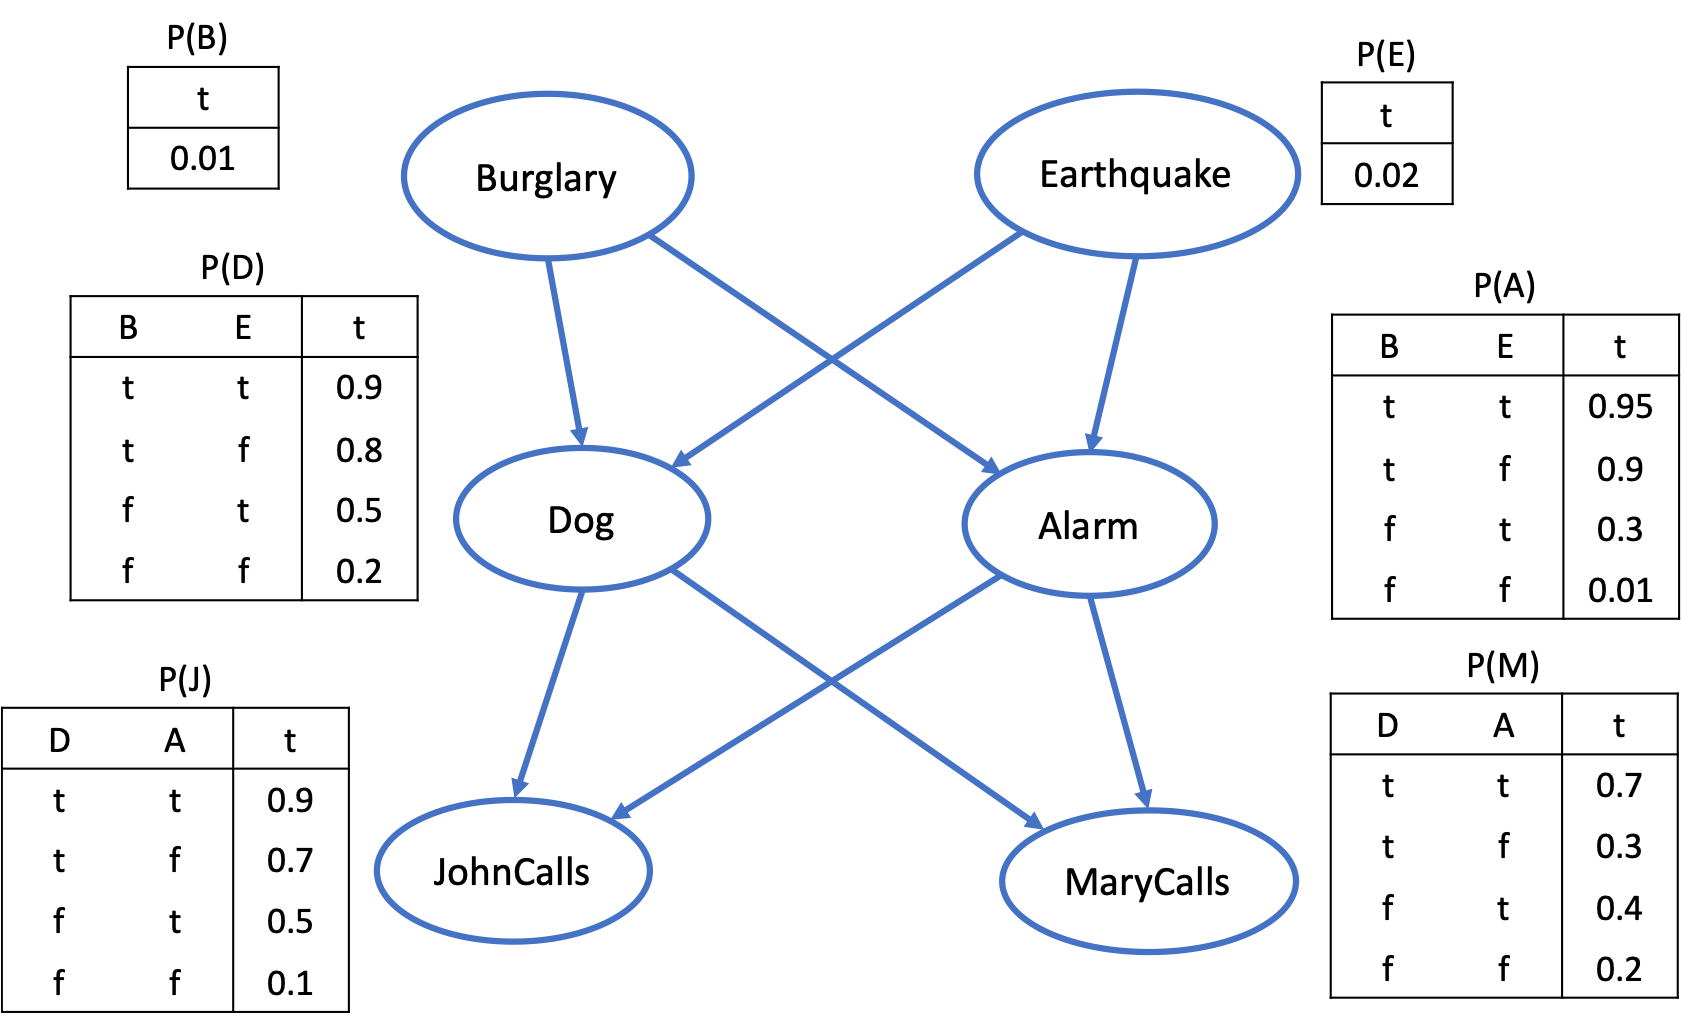
\includegraphics[scale=0.5]{p1}
\label{fig:q1}
\end{figure}

\begin{soln}
\begin{equation}
\begin{split}
P(d|b,\neg a,j,m) & = \frac{P(d,b,\neg a,j,m,E)}{P(D,b,\neg a,j,m,E)}\\
&= \frac{\sum\limits_{e,\neg e}P(d,b,\neg a,j,m,E)}{\sum\limits_{d, \neg d, e,\neg e}P(D,b,\neg a,j,m,E)}\\
&= \frac{\sum\limits_{e,\neg e}P(b)P(E)P(d|b,E)P(\neg a|b,E)P(j|d,\neg a)P(m|d,\neg a)}{\sum\limits_{d, \neg d, e,\neg e}P(b)P(E)P(D|b,E)P(\neg a|b,E)P(j|D,\neg a)P(m|D,\neg a)}\\
&= (0.01\times0.02\times0.9\times0.05\times0.7\times0.3+0.01\times0.98\times0.8\times0.1\times0.7\times0.3)\\
&\quad/(0.01\times0.02\times0.9\times0.05\times0.7\times0.3+0.01\times0.98\times0.8\times0.1\times0.7\times0.3\\
&\quad+0.01\times0.02\times0.1\times0.05\times0.1\times0.2+0.01\times0.98\times0.2\times0.1\times0.1\times0.2)\\
&=0.9769
\end{split}
\end{equation}
\end{soln}

\pagebreak


\item Given the following Bayesian network and sample counts in each table, where sample counts \texttt{<n\textsubscript{true}, n\textsubscript{false}>}, there are \texttt{n\textsubscript{true}} samples with true labels and \texttt{n\textsubscript{false}} samples with false labels for this attribute. For example, \texttt{<138, 132>} in table \texttt{C|A} says given the condition of $A = true$, there are 138 instances are true and 132 are false with regard to attribute $C$.

You need to answer the following two questions.


\begin{figure}[H]
\centering
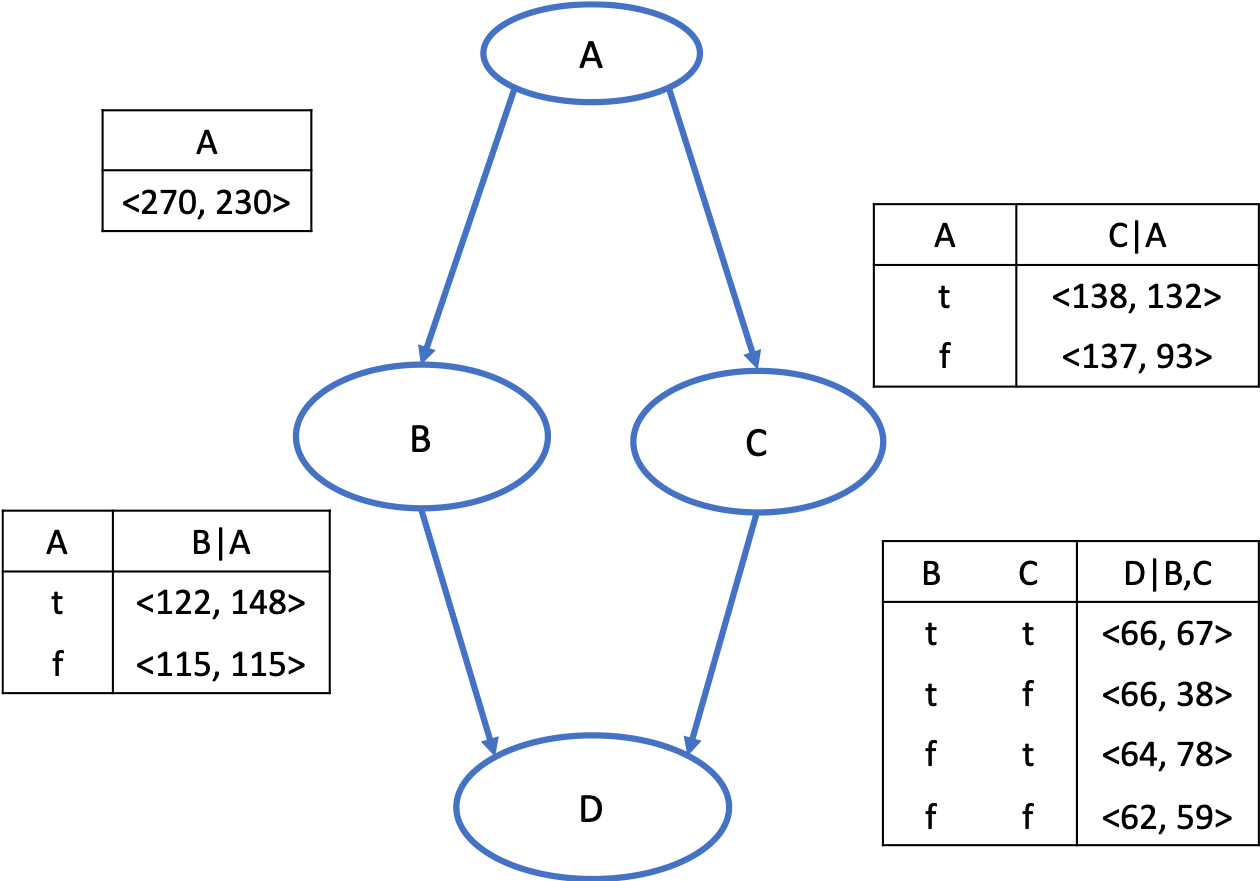
\includegraphics[scale=0.5]{p2}
\label{fig:q2}
\end{figure}


\begin{enumerate}
\item (2 pts) Construct the conditional probability tables (CPTs) based on the above sample count tables, using maximum likelihood estimation. You need to both show the true probability \texttt{P\textsubscript{true}} and false probability P\textsubscript{false} for each case, and organize them in the format of \texttt{<P\textsubscript{true}, P\textsubscript{false}>}. For example, for the case \texttt{Y|X\textsubscript{1},X\textsubscript{2}}, your answer will look like \texttt{<P(Y|X\textsubscript{1},X\textsubscript{2}), P($\neg$Y|X\textsubscript{1},X\textsubscript{2})>}. Keep \textbf{at least 3 digits of precision.} (You may reuse the same structure as the above tables, just plugging in the conditional probabilities in the place of sample counts. For more information, please refer to the lecture notes \texttt{BNs-1.pdf})

\begin{soln}
Since we are only given a set of data. Using maximum likelihood estimation to estimate CPTs is equivalently to calculate CPTs from distribution of data sets and also, we can independently calculate each CPT:\\
$P(A) = <\frac{270}{500},\frac{230}{500}>=<0.540,0.460>$
\begin{tabular}{|c|}
\hline
A                                    \\ \hline
\textless{}0.540,0.460\textgreater{} \\ \hline
\end{tabular}\\
For $P(B|A)$:
\begin{tabular}{|c|c|}
\hline
A & B$|$A                                  \\ \hline
t & \textless{}0.415,0.548\textgreater{} \\ 
f & \textless{}0.500,0.500\textgreater{} \\ \hline
\end{tabular}\\
For $P(C|A)$:
\begin{tabular}{|c|c|}
\hline
A & C$|$A                                  \\ \hline
t & \textless{}0.511,0.489\textgreater{} \\ 
f & \textless{}0.596,0.404\textgreater{} \\ \hline
\end{tabular}\\
For $P(D|B,C)$:
\begin{tabular}{|c|c|}
\hline
B    C   & D$|$B,C                              \\ \hline
t      t & \textless{}0.496,0.504\textgreater{} \\ 
t      f & \textless{}0.635,0.365\textgreater{} \\ 
f      t & \textless{}0.451,0.549\textgreater{} \\ 
f      f & \textless{}0.512,0.288\textgreater{} \\  \hline
\end{tabular}\end{soln}

\vspace{10pt}

\item (10 pts) Show the result of one cycle of the EM algorithm to update the CPTs you derived in step (a), using 10 another instances with \texttt{A=true}, \texttt{B=false}, \texttt{C=?}, and \texttt{D=true} (`?' means missing value). Keep \textbf{at least 2 digits of precision}.

\begin{soln}
E-step:\\
According to CPTs from part(a), 
\begin{equation}
\begin{split}
P(c|a,\neg b,d) &= \frac{P(c, a,\neg b,d)}{P(c|a,\neg b,d)+P(\neg c|a,\neg b,d)} \\
& = \frac{P(a)P(c|a)P(\neg b|a)P(d|c,\neg b)}{P(a)P(c|a)P(\neg b|a)P(d|c,\neg b)+P(a)P(\neg c|a)P(\neg b|a)P(d|\neg c,\neg b)}\\
& = \frac{0.540\times0.511\times0.500\times0.451}{0.540\times0.511\times0.500\times0.451+0.540\times0.489\times0.500\times0.512}\\
& = 0.479
\end{split}
\end{equation}
correspondingly:
\begin{equation}
P(\neg c|a,\neg b,d) = 0.521
\end{equation}
\begin{tabular}{|llll|}
\hline
A & B & C                                                         & D \\ \hline
t & f & \begin{tabular}[c]{@{}l@{}}t:0.479\\ f:0.521\end{tabular} & t \\ 
t & f & \begin{tabular}[c]{@{}l@{}}t:0.479\\ f:0.521\end{tabular} & t \\ 
t & f & \begin{tabular}[c]{@{}l@{}}t:0.479\\ f:0.521\end{tabular} & t \\ 
t & f & \begin{tabular}[c]{@{}l@{}}t:0.479\\ f:0.521\end{tabular} & t \\ 
t & f & \begin{tabular}[c]{@{}l@{}}t:0.479\\ f:0.521\end{tabular} & t \\ 
t & f & \begin{tabular}[c]{@{}l@{}}t:0.479\\ f:0.521\end{tabular} & t \\ 
t & f & \begin{tabular}[c]{@{}l@{}}t:0.479\\ f:0.521\end{tabular} & t \\ 
t & f & \begin{tabular}[c]{@{}l@{}}t:0.479\\ f:0.521\end{tabular} & t \\ 
t & f & \begin{tabular}[c]{@{}l@{}}t:0.479\\ f:0.521\end{tabular} & t \\ \hline
\end{tabular}

M-step:
Restimate the CPTs according to data distribution and here is new distribution:\\
\begin{tabular}{|c|}
\hline
A                                    \\ \hline
\textless{}280,230\textgreater{} \\ \hline
\end{tabular}
\begin{tabular}{|c|c|}
\hline
A & B$|$A                                  \\ \hline
t & \textless{}122,158\textgreater{} \\ 
f & \textless{}115,115\textgreater{} \\ \hline
\end{tabular}
\begin{tabular}{|c|c|}
\hline
A & C$|$A                                  \\ \hline
t & \textless{}142.79,137.21\textgreater{} \\ 
f & \textless{}137,93\textgreater{} \\ \hline
\end{tabular}
\begin{tabular}{|c|c|}
\hline
B    C   & D$|$B,C                              \\ \hline
t      t & \textless{}66,67\textgreater{} \\ 
t      f & \textless{}66,38\textgreater{} \\ 
f      t & \textless{}68.79,78\textgreater{} \\ 
f      f & \textless{}67.21,59\textgreater{} \\  \hline
\end{tabular}\\
The corresponding CPTs:\\
\begin{tabular}{|c|}
\hline
A                                    \\ \hline
\textless{}0.549,0.451\textgreater{} \\ \hline
\end{tabular}
\begin{tabular}{|c|c|}
\hline
A & B$|$A                                  \\ \hline
t & \textless{}0.436,0.564\textgreater{} \\ 
f & \textless{}0.500,0.500\textgreater{} \\ \hline
\end{tabular}
\begin{tabular}{|c|c|}
\hline
A & C$|$A                                  \\ \hline
t & \textless{}0.510,0.490\textgreater{} \\ 
f & \textless{}0.596,404\textgreater{} \\ \hline
\end{tabular}
\begin{tabular}{|c|c|}
\hline
B    C   & D$|$B,C                              \\ \hline
t      t & \textless{}0.496,0.504\textgreater{} \\ 
t      f & \textless{}0.635,365\textgreater{} \\ 
f      t & \textless{}0.469,0.531\textgreater{} \\ 
f      f & \textless{}0.533,0.467\textgreater{} \\  \hline
\end{tabular}
\end{soln}

\section*{Part 2}
\begin{soln}

\begin{figure}[h]
\centering

\includegraphics[scale=1]{../pr}
\label{fig:pr}
\end{figure}


I think TAN seems to have more predictive power, since the area under the TAN curve is larger than the area under NB curve. In another words, TAN curve is more close to point(recall=1, precision=1).\\

\section*{Part 3}
I shuffled the data before 10-fold cross validation:\\
The sample mean for NB is 0.693.\\
The sample mean for TAN is 0.759.\\
$t$-value is 6.654.\\
The corresponding $t$-value for a two-tailed $t$-test at $p=0.05$ and degrees of freedom = 9 is  2.262. Obtained $t$-value is larger than 2.262. Thus two systems seem to provide different accuracies.(TAN is better). \\
We can also calculate $p$-value corresponding to $t$=6.654, which is 0.000093, much smaller than 0.5.
\end{soln}


\end{enumerate}
\end{enumerate}


\end{document}
